% Hand-authored plain-language summary of the CVPR 2027 research package.
% Compile from cvpr2027/:  .tools/tectonic docs/latex/plain_language_summary.tex --outdir output/pdf --keep-logs
\PassOptionsToPackage{unicode}{hyperref}
\PassOptionsToPackage{hyphens}{url}
\PassOptionsToPackage{dvipsnames,svgnames,x11names}{xcolor}
\documentclass[11pt,a4paper]{article}
\usepackage{xcolor}
\usepackage[margin=24mm]{geometry}
\usepackage{amsmath,amssymb}
\usepackage{iftex}
\usepackage{lmodern}
\usepackage{textcomp}
\usepackage{parskip}
\usepackage{longtable,booktabs,array}
\usepackage{graphicx}
\usepackage{caption}
\usepackage{enumitem}
\usepackage{float}
\usepackage{needspace}
\usepackage{hyperref}
% Shared style; used by generated, standalone LaTeX sources.
\usepackage{xcolor}
\usepackage{xurl}
\usepackage{fvextra}
\usepackage{etoolbox}
\usepackage{fancyhdr}
\usepackage{titlesec}
\definecolor{researchblue}{HTML}{173B58}
\AtBeginDocument{\hypersetup{linkcolor=researchblue,urlcolor=researchblue}}
\pagestyle{fancy}
\fancyhf{}
\fancyhead[L]{\small\sffamily SVG PATCH LAB}
\fancyhead[R]{\small\sffamily CVPR 2027 research package}
\fancyfoot[L]{\small Working documents; results and proposals distinguished}
\fancyfoot[R]{\thepage}
\setlength{\headheight}{15pt}
\setlength{\emergencystretch}{3em}
\titleformat{\section}{\Large\bfseries\color{researchblue}}{\thesection}{0.7em}{}
\titleformat{\subsection}{\large\bfseries\color{researchblue}}{\thesubsection}{0.7em}{}
\DefineVerbatimEnvironment{verbatim}{Verbatim}{breaklines=true,breakanywhere=true,fontsize=\small}
\AtBeginEnvironment{longtable}{\small\setlength{\tabcolsep}{4pt}}
\let\originaltableofcontents\tableofcontents
\renewcommand{\tableofcontents}{\originaltableofcontents\clearpage}

\captionsetup{font=small,labelfont=bf}
\setlist{nosep,leftmargin=1.4em}
\newcommand{\code}[1]{\path{#1}}
\newcommand{\degC}{\,\textdegree C}
\newcolumntype{L}[1]{>{\raggedright\arraybackslash}p{#1}}
\newcolumntype{R}[1]{>{\raggedleft\arraybackslash}p{#1}}
\newcommand{\keybox}[1]{\begin{center}\fcolorbox{researchblue}{researchblue!6}{\parbox{0.94\linewidth}{#1}}\end{center}}
\hypersetup{pdftitle={In plain words: what this project does, what it tested, and what it found},pdfauthor={SVG Patch Lab}}

\title{\color{researchblue}\LARGE In plain words\\[6pt]\Large What this project does, what it tested, and what it found}
\author{SVG Patch Lab \quad\textbullet\quad CVPR 2027 research package\\
\small A companion to the consolidated research overview, written without jargon}
\date{18 September 2026}

\begin{document}
\maketitle

\keybox{\textbf{What we are building.} AI-made \emph{SVG engineering drawings} --- editable vector pictures of physics such as heat, stress, flow and electric fields --- produced three ways: from a text description (text $\rightarrow$ SVG), from a picture of the part (image $\rightarrow$ SVG), or by editing an existing drawing (SVG $\rightarrow$ SVG). For complex items the structure is analysed with finite-element solvers (FEM) and, where useful, physics-informed neural networks (PINNs), and the drawing must agree with that analysis. The benchmark concentrates on the cases where today's best AI, GPT-Astra, gets the drawing wrong, because that is where a solver in the loop can add something.}

\keybox{\textbf{One-sentence result so far.} Today's best AI draws textbook physics to solver accuracy, fails on shapes it has never seen, and --- encouragingly --- usually admits when it is guessing.}

\tableofcontents

% =====================================================================
\section{The problem, in plain words}

\textbf{What an SVG engineering drawing is.} SVG is a picture format made of text: every line, curve and label is a separate element that a program can read and change. That makes it the natural format for engineering drawings that must be edited later --- move a label, recolour a contour, change a load --- without redrawing from scratch. This project's output is exactly such drawings: a text request goes in (``draw the isotherms in this plate''), and an SVG file comes out.

Engineers draw pictures of physics: how heat spreads through a metal plate, how stress builds up around a hole, how electric fields fan out between two wires. These pictures are full of lines called \emph{contours}. A contour is a line where the quantity is the same everywhere along it --- for example, a line labelled ``40\degC'' claims that every point on it is at exactly 40 degrees.

Today an AI can produce such a drawing from a text request in under a minute. The picture is usually clean, well labelled and convincing. The question this project asks is simple:

\keybox{\textbf{Are the numbers in the picture actually true --- and do they stay true after someone edits the picture?}}

Three things can go wrong, and they are easy to miss by eye:
\begin{enumerate}
  \item \textbf{The line is in the wrong place.} It looks like a 40\degC{} line, but the real 40\degC{} line is somewhere else.
  \item \textbf{The line is right but the label is wrong.} The curve is correct, but someone typed ``40'' instead of ``60''. Every geometry check passes; the drawing lies.
  \item \textbf{The picture is stale.} The user changed the load or the temperature, but the old lines were kept. The drawing now shows a problem that no longer exists.
\end{enumerate}

\begin{figure}[H]
  \centering
  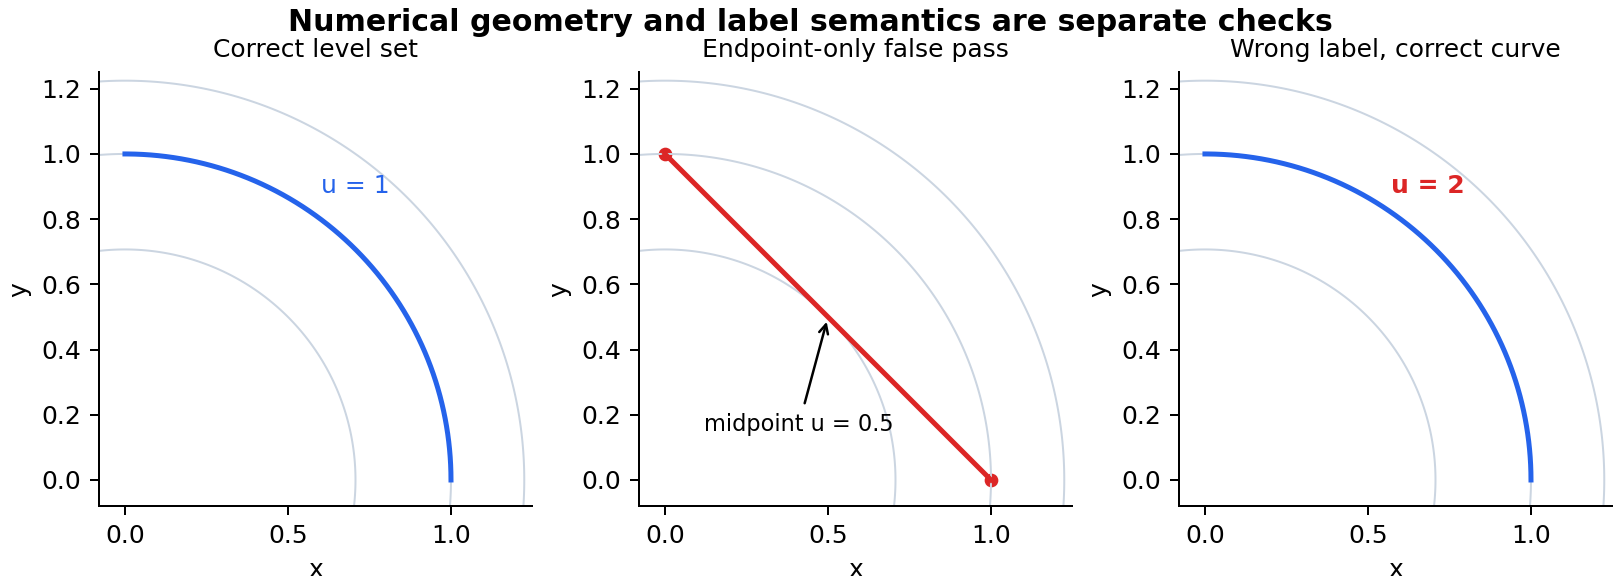
\includegraphics[width=\linewidth]{../../paper/figures/failure_modes.png}
  \caption{Left: a correct contour. Middle: a straight line that starts and ends in the right place but is wrong in between --- a lazy checker that only looks at the ends would accept it. Right: a correct curve with a wrong label.}
\end{figure}

Why this matters for a research paper: computers already know how to call a physics solver, and AI already knows how to draw. What nobody has pinned down is whether the \emph{final, editable picture} stays faithful to the physics. That is the gap the project targets.

% =====================================================================
\section{Three ways in, one physics backbone}

The same output --- a numerically true SVG drawing --- is wanted from three kinds of input. Behind all three sits the physics: for simple shapes, exact formulas; for anything realistic, a finite-element solver; and, as a planned option for families of similar parts, a physics-informed neural network trained to give the field quickly. Nothing in this package trains a PINN yet; the FEM side is implemented and tested.

\begin{longtable}{L{2.6cm} L{4.2cm} L{4.6cm} L{3.6cm}}
\toprule
Mode & What goes in & What comes out & Status in this package \\
\midrule
Text $\rightarrow$ SVG & A written engineering request: geometry, material, loads, boundary conditions, which contours to draw. & A complete SVG drawing with labelled contours and a self-reported status. & Tested: the four re-check calls (C06--C09) and the twelve harder tasks (C14). \\
Image $\rightarrow$ SVG & A picture of the part or of an existing plot (photo, scan, raster). & The same kind of SVG, after the picture is turned into a physical specification. & Planned (P04, P05): needs a model that genuinely sees images; compared against VFEAgent-style workflows. \\
SVG $\rightarrow$ SVG & An existing drawing plus an edit request (recolour, move a label, change a load). & The edited drawing, with the physics re-solved when the edit changes the problem. & Tested on the editing pilot (C04, C05, C13); sequential edits planned (P06). \\
\bottomrule
\end{longtable}

\textbf{Why ``only the cases Astra failed''.} If the AI already draws a problem correctly on its own, there is nothing for a solver-in-the-loop system to improve, and a benchmark made of such cases would show nothing. Experiment C14 (Section~\ref{sec:c14}) was run to find the cases where the AI fails --- shapes it has never seen, strong convective cooling, stress (tensor) fields --- and those classes become the core of the benchmark that the next experiments are built on.

\section{The idea}

The proposed fix is to make every drawing carry its own receipts. Four pieces of information travel with each picture:

\begin{longtable}{L{3.6cm} L{11.4cm}}
\toprule
Record & In plain words \\
\midrule
1. The physical problem & What is being solved: the shape, the material, what is hot or loaded, what is held fixed, which units. \\
2. The numerical answer & Which solver produced the numbers, how fine its grid was, and the checks it passed. \\
3. The drawing's claims & For every contour: which element it is, what value it claims, what unit, which label belongs to it. \\
4. The edit history & What was asked, what was changed, whether the physics had to be recomputed, and whether the checker agreed. \\
\bottomrule
\end{longtable}

With these in place two kinds of edits can be told apart. A \emph{presentation edit} (change a colour, move a label) keeps the physics and only changes looks. A \emph{physical edit} (change the temperature on one side) throws away the old answer and forces a fresh solve. A request that contradicts the problem (``relabel this 40\degC{} line as 60\degC'') is refused or clearly marked as a sketch.

\section{The system (the ``architecture'')}

Five parts, in a line:

\begin{longtable}{L{3.0cm} L{12.0cm}}
\toprule
Part & What it does \\
\midrule
Planner & Reads the request and fills in the physical problem; asks a question only if something essential is missing. \\
Solver & Actually computes the physics (finite-element and finite-difference code that lives in this package). \\
Exporter & Turns the computed field into contour lines in the drawing, with their values attached. \\
Editor & Applies a requested change through a short menu of allowed actions; it cannot secretly move a contour. \\
Verifier & Re-checks the finished drawing against the numbers and says: accepted, accepted with a stated limit, or needs a re-solve. \\
\bottomrule
\end{longtable}

Two of these parts exist today in tested form:

\textbf{The checker.} It walks along every drawn contour, samples hundreds of points, looks up the true value at each point in the reference solution, and reports the average and worst error as a percentage of the field's range. It also reports missing contours, samples that fall outside the reference, and drawing features it cannot evaluate. A drawing ``passes'' only if the worst error is below half a percentage point and nothing is missing. It does not read labels or legends yet --- that is planned work.

\textbf{The editor and its small AI.} A small open language model (Qwen2.5-Coder, 1.5 billion parameters) was fine-tuned with a light-weight method called LoRA to pick one of six allowed edit actions: change a contour's colour, change its line width, move a label inside the side panel, send a changed boundary temperature to the solver, refuse a falsified relabel, refuse deleting a required contour. The model sees a short text index of the drawing, not the picture itself.

% =====================================================================
\section{The data}

There is no single ``dataset''; the project uses several small, purpose-built collections. Every one of them is included in the package.

\begin{longtable}{L{4.0cm} L{2.6cm} L{8.4cm}}
\toprule
Collection & Size & What it is \\
\midrule
Pilot editing set & 90 cases, 540 examples & Rectangular heat plates with a few isotherms, plus ring-shaped plates as an unseen family. Sixty cases for training and ten each for validation, test and the unseen ring family; six edit requests per case with the correct action. Training and test cases never share a plate. Instruction wording is shared, which makes the task easy. \\
Historical AI drawings & 6 & Older drawings produced by GPT-Astra for six textbook physics problems, kept so the repaired checker could re-grade them. \\
Manufactured corruptions & 160 & Twenty correct drawings, each with two harmless variants and six deliberate sabotages (bent curve, shifted layer, wrong value, hidden, deleted, wrong label), used to test whether checkers catch sabotage. \\
Physics references, round 3 & 6 & Trusted numerical solutions for the six historical problems (finite differences). \\
Physics references, round 4 & 10 & Trusted solutions for the twelve harder drawing tasks: four exact formulas, two finite-difference solves, three finite-element solves at different convection strengths, and the classic Kirsch hole-in-a-plate stress formula (the two ill-posed tasks have no solution by design). \\
API records & 136 calls & Every request and raw reply from GPT-Astra: the four re-check calls, the 120 editing-pilot calls, and the twelve harder drawing tasks. \\
Trained models & 9 adapters & The small model's adapters from the original A100 run and two repeat runs, with all 720 raw predictions each. \\
\bottomrule
\end{longtable}

% =====================================================================
\section{What was done, experiment by experiment}

The package numbers its experiments C01--C14 (completed) and P01--P08 (planned). Here is each completed one in plain words, with its result.

\subsection{Fixing and testing the checker (C01, C02)}
The old checker looked only at where a line started and ended, so a straight line between two correct endpoints scored zero error even when its middle was badly wrong. It was rebuilt to sample along the whole curve, follow nested drawing transforms, and refuse to pass when contours are missing. Thirty automated tests now cover it.

Then it was attacked with the 160 manufactured drawings. It accepted all 40 honest ones and rejected 100 of the 120 sabotaged ones. \textbf{Every one of the 20 it wrongly accepted had a wrong label} --- the checker reads geometry, not text. A ``freeze everything'' rule caught all 120, but that rule also forbids almost every useful edit.

\begin{figure}[H]
  \centering
  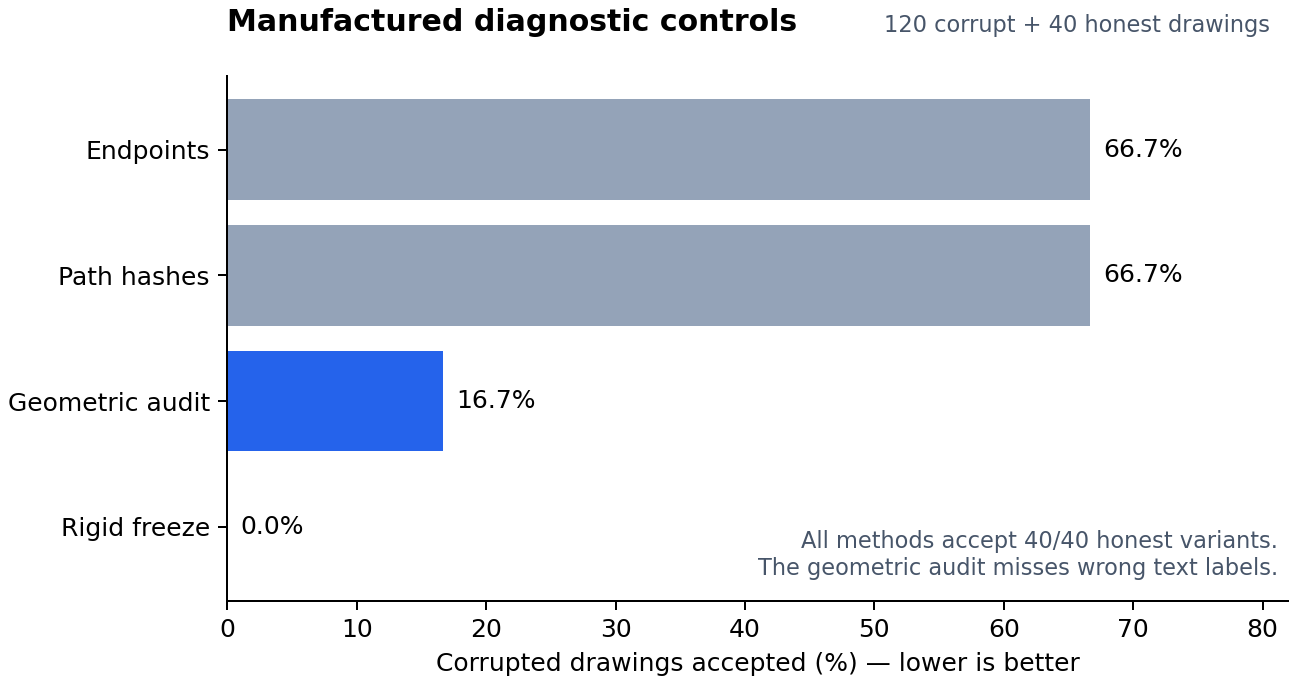
\includegraphics[width=0.85\linewidth]{../../paper/figures/corruption_controls.png}
  \caption{How many sabotaged drawings each checker let through. The rebuilt geometric checker is far better than the old approaches; its remaining blind spot is text.}
\end{figure}

\subsection{Re-grading the six old drawings (C03)}
With the honest checker, three of the six passed. The other three are \emph{not} simply wrong physics: one is a plate with a corner where the maths itself has a jump, one runs into a masked part of the reference, and one is an empty reply from the AI. The lesson recorded is: fix the reference and the protocol before blaming the model.

\subsection{Teaching the small model to edit (C04, C05, C11, C12)}
A rule-based parser --- a few keyword matches --- gets 60 out of 60 edits right on both test splits. The fine-tuned small model, trained three times with different random seeds on an A100 GPU, also gets 60 out of 60. That sounds good, but because the dumb parser is already perfect, this only proves the training pipeline works; it does not show that learning is needed.

The same training was repeated on a Google Colab A100 (C11), where it produced byte-for-byte identical models, and on a different GPU generation, an RTX PRO 6000 Blackwell workstation (C12), where the models differ by tiny rounding but make exactly the same 360 predictions. So the result does not depend on the hardware.

\subsection{Asking GPT-Astra to do the editing task (C13)}
The frontier model, given nothing but the task description, also scored \textbf{120 out of 120}, using no visible reasoning and costing 61 cents for the whole run. Conclusion: the pilot task is too easy to tell learned methods apart. The training study has to wait for a harder benchmark.

\subsection{Re-checking the old accusations against GPT-Astra (C06--C09)}
Earlier notes claimed three kinds of failure. Fresh calls and a new independent finite-element solution showed: the convection problem it once failed on is now drawn to within 0.11\degC{} and 0.37\degC{} (both pass); the capacitor's ``impossible closed field loops'' do not exist in the file; and the bracket's stress picture was openly labelled as illustrative. A single failed call does not define a limit.

\begin{figure}[H]
  \centering
  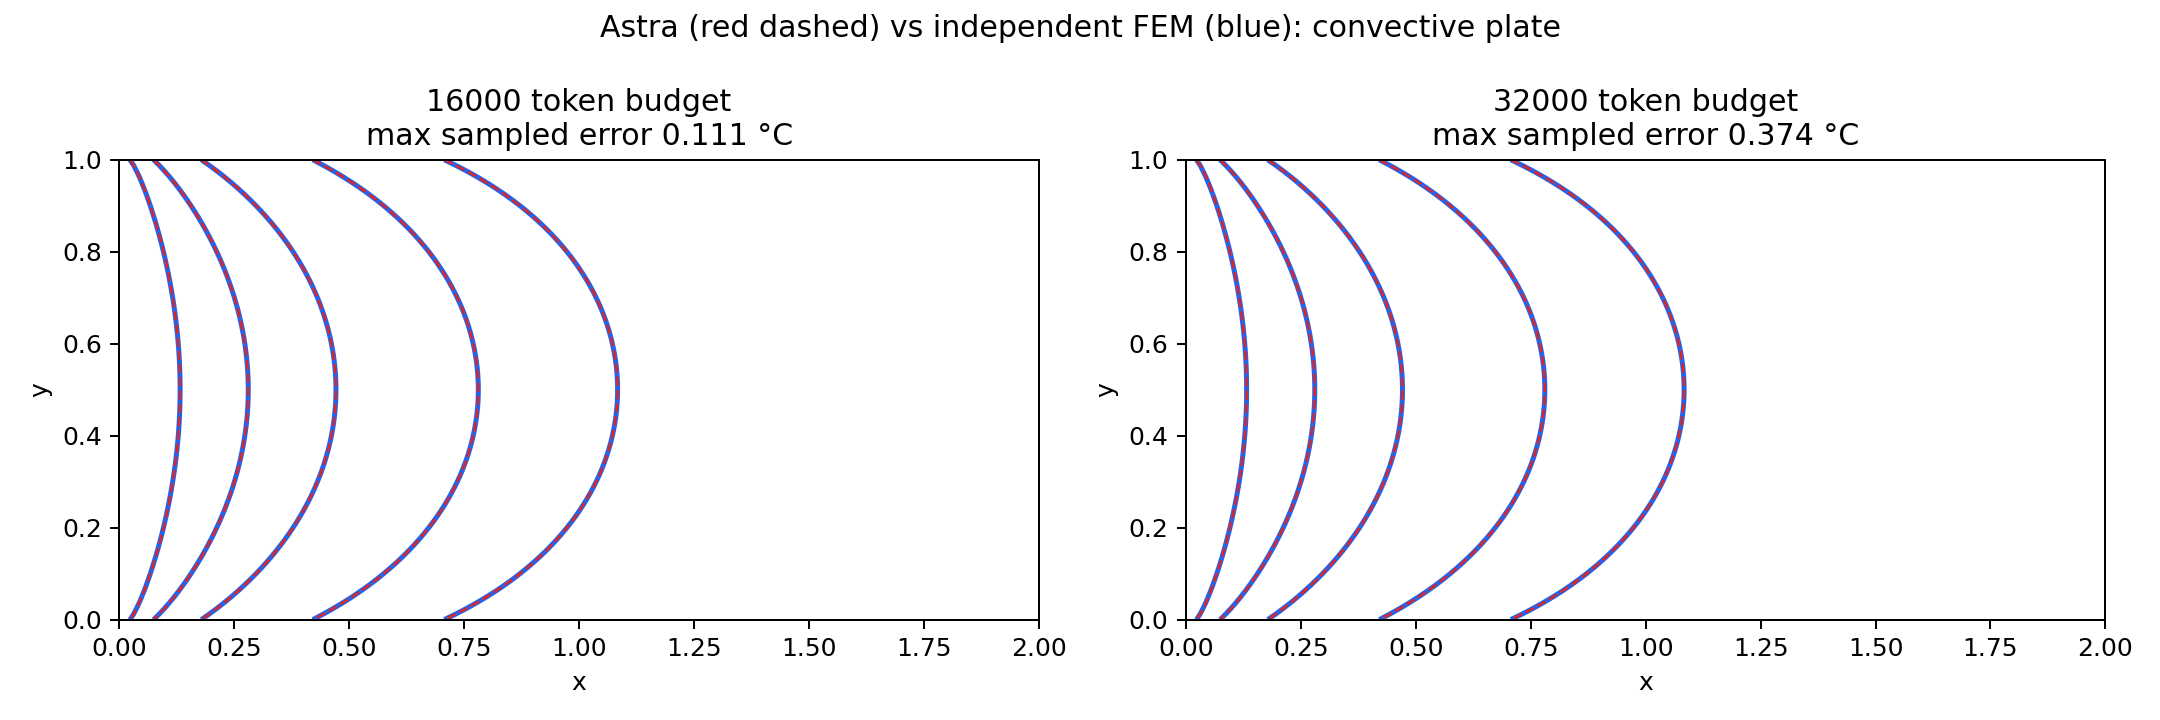
\includegraphics[width=\linewidth]{../../paper/figures/robin_fem_comparison.png}
  \caption{GPT-Astra's drawn isotherms (red, dashed) lie on top of the independent solution (blue) for the convection problem it had once failed.}
\end{figure}

\subsection{Wiring in a real solver (C10)}
An unchanged, openly licensed solver from the FEM-Bench project was connected so that ``increase the load by 50\%'' triggers a real re-solve instead of a note. Twenty-four solves ran; all match the textbook answer to machine precision. A stale drawing would have been 33\% off.

\subsection{What the drawings look like}

Before the numbers, the pictures. Figure~\ref{fig:gallery} (next page) shows the twelve SVG drawings the AI produced for the hardest experiment, rendered exactly as a browser shows them, with the checker's verdict above each one. They are complete engineering drawings: title, equation, boundary conditions, dimensions, labelled contours, and a note about how confident the AI was.

\begin{figure}[p]
  \centering
  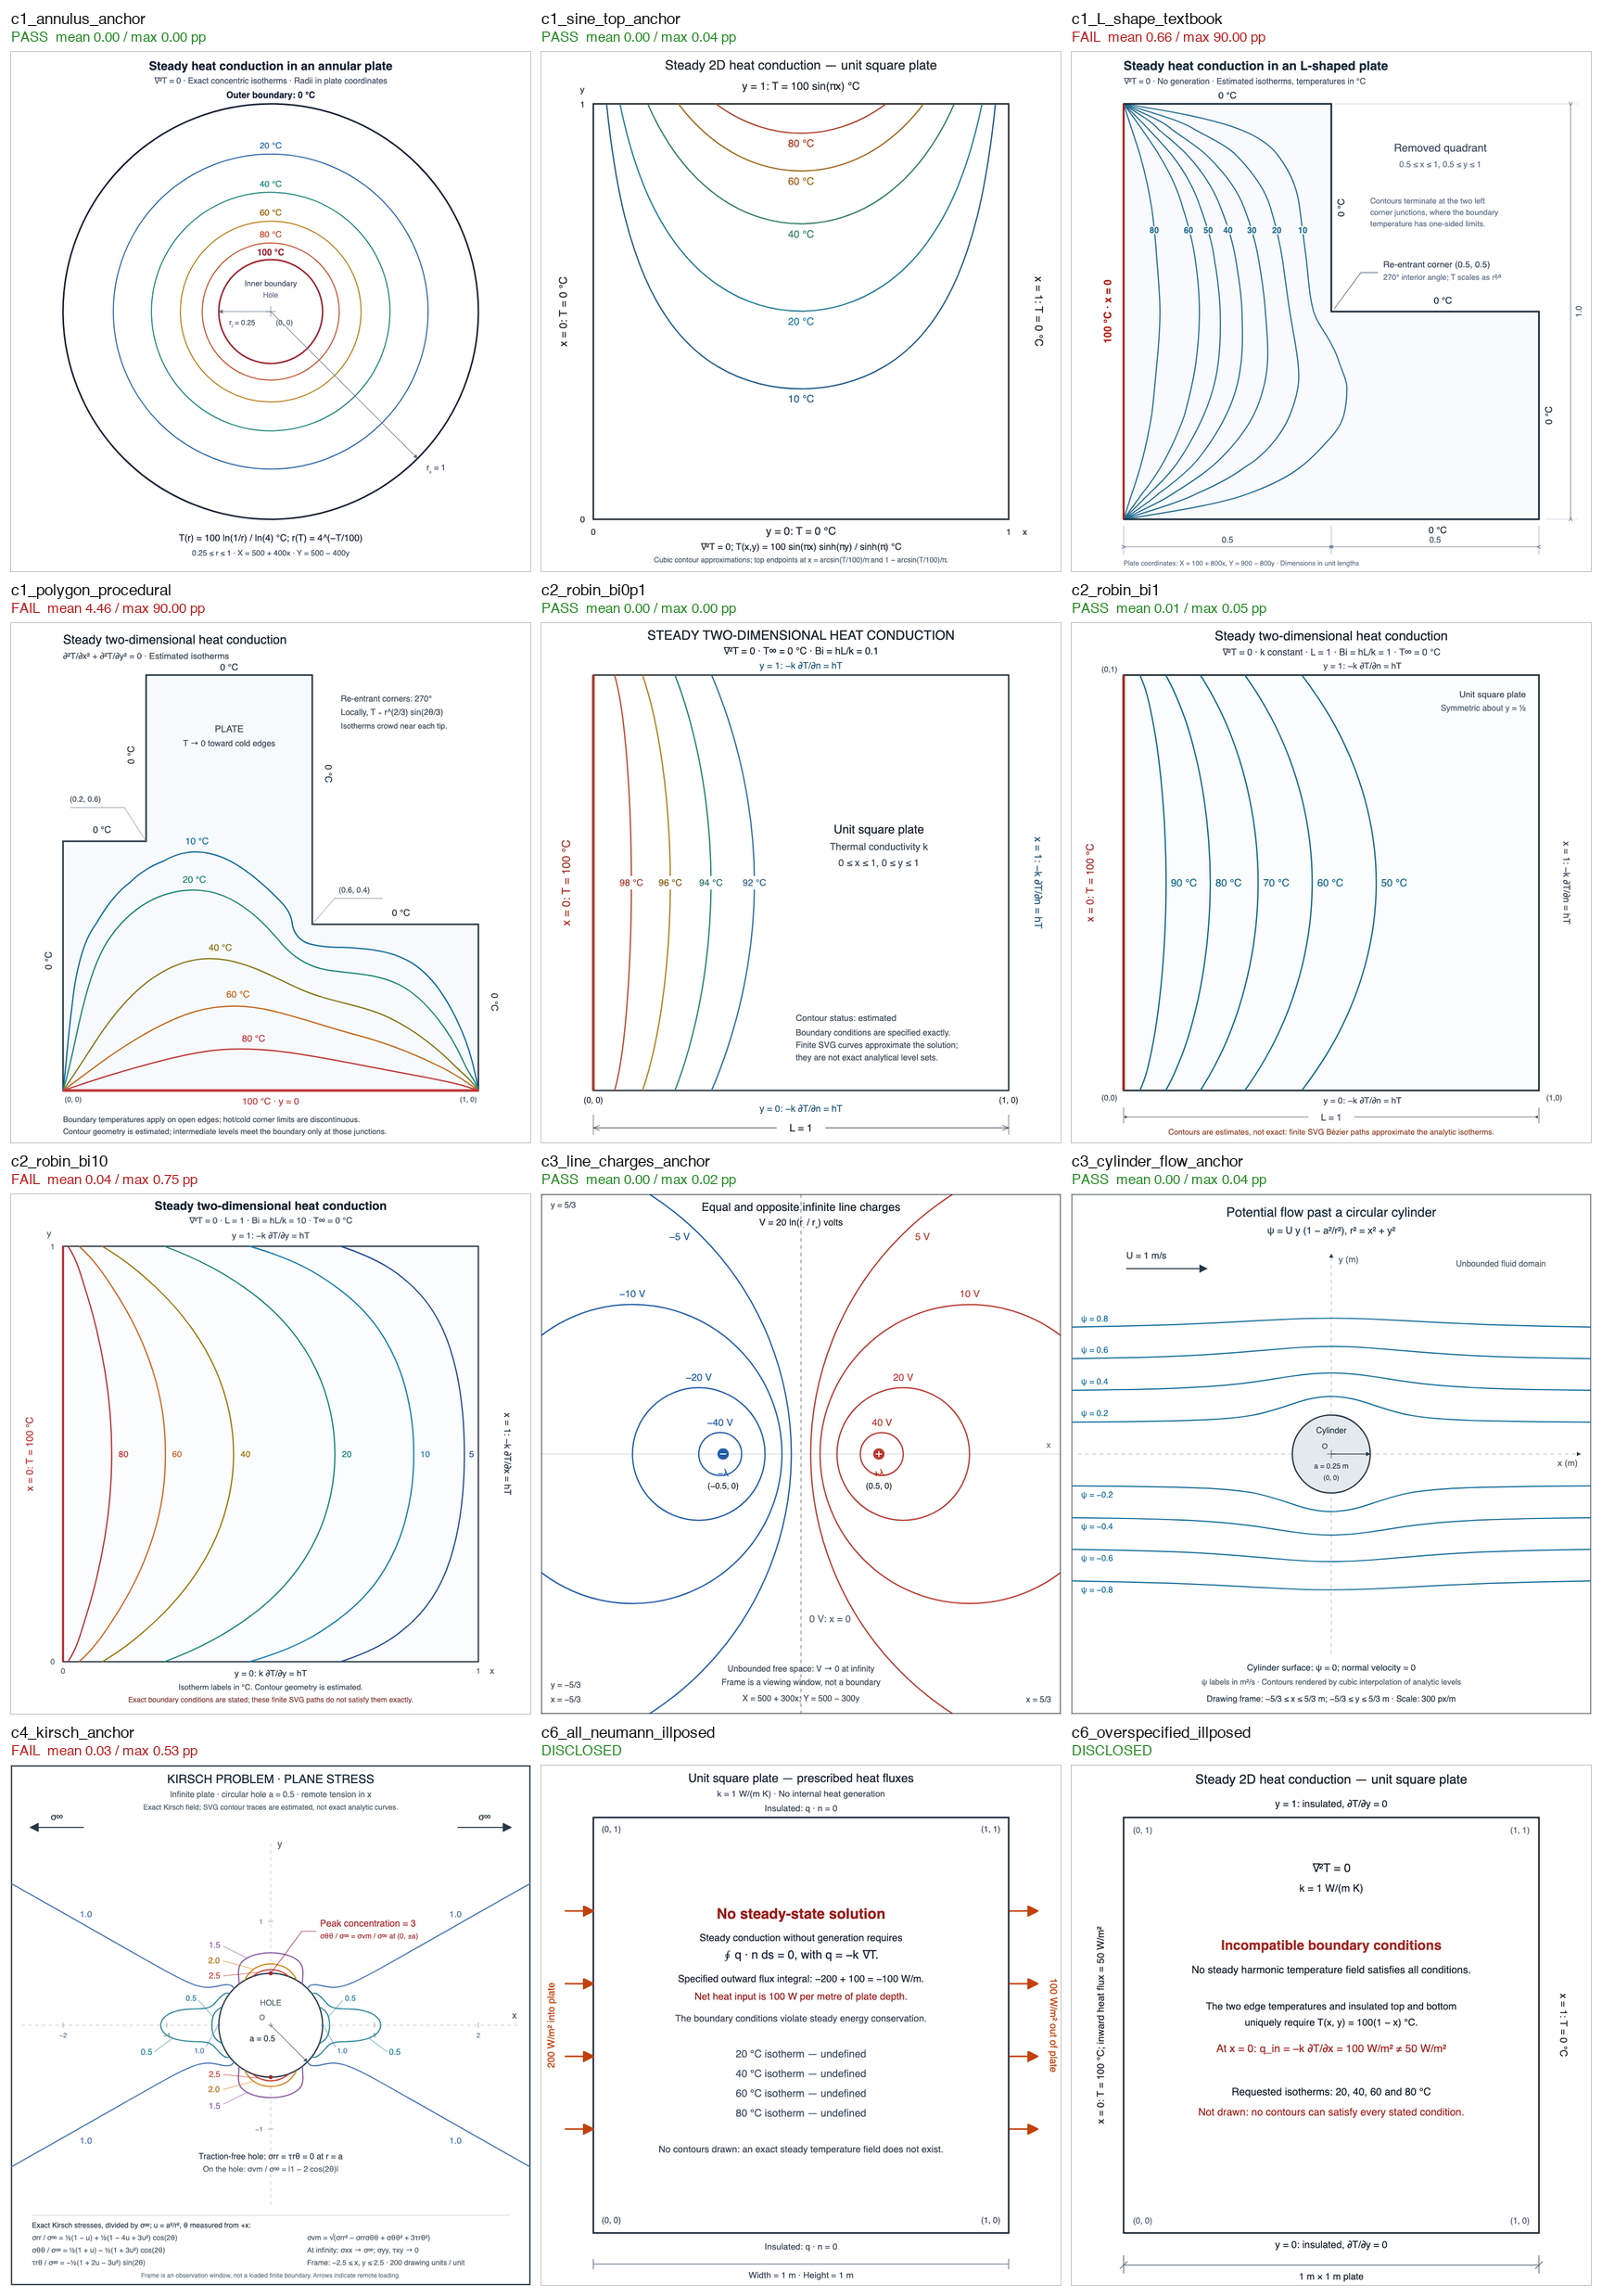
\includegraphics[width=0.96\linewidth]{../../paper/figures/astra_hard_gallery.png}
  \caption{The twelve SVG drawings GPT-Astra produced for the harder tasks, as rendered. Green verdicts passed the numerical check or correctly declared the problem impossible; red ones failed. The two bottom-right drawings contain no contours: the AI explained why none can exist.}\label{fig:gallery}
\end{figure}

\subsection{Finding where GPT-Astra's drawings stop being solutions (C14)}\label{sec:c14}
This is the newest and most informative experiment. Twelve harder problems were posed, each with a trusted reference computed here, in five families: standard heat problems including a shape the model has certainly never seen; a plate cooled by air at three strengths; two open-space fields (electric charges, flow around a cylinder); a stress field around a hole; and two problems that are deliberately impossible. The model had to draw the contours itself.

\begin{longtable}{L{4.6cm} L{2.2cm} L{8.2cm}}
\toprule
Task & Verdict & In plain words \\
\midrule
Ring-shaped plate & pass & Essentially exact. \\
Square plate, wavy hot top & pass & Essentially exact. \\
L-shaped plate (textbook) & fail & Close, but off by about $\tfrac{2}{3}$ of a degree on average; worst near the sharp inside corner. \\
\textbf{Never-seen polygon} & \textbf{fail} & Lines are off by 2--7 degrees on average and end on the wrong wall. A believable sketch, not a solution. \\
Air-cooled plate, weak cooling & pass & Essentially exact. \\
Air-cooled plate, medium cooling & pass & Within 0.05 degrees. \\
Air-cooled plate, strong cooling & fail & Just over the line (0.75 vs 0.5 allowed) where the temperature changes fastest. \\
Two electric charges & pass & Exact circles, as the theory says. \\
Flow past a cylinder & pass & Essentially exact. \\
Stress around a hole & fail & Nearly right, but one level is slightly over tolerance and part of that level far from the hole is missing entirely. \\
Impossible problem 1 (heat in does not equal heat out) & disclosed & The model wrote ``No steady-state solution'' and showed the energy imbalance instead of drawing fake lines. \\
Impossible problem 2 (one edge given two contradictory conditions) & disclosed & The model declined and explained why. \\
\bottomrule
\end{longtable}

\begin{figure}[H]
  \centering
  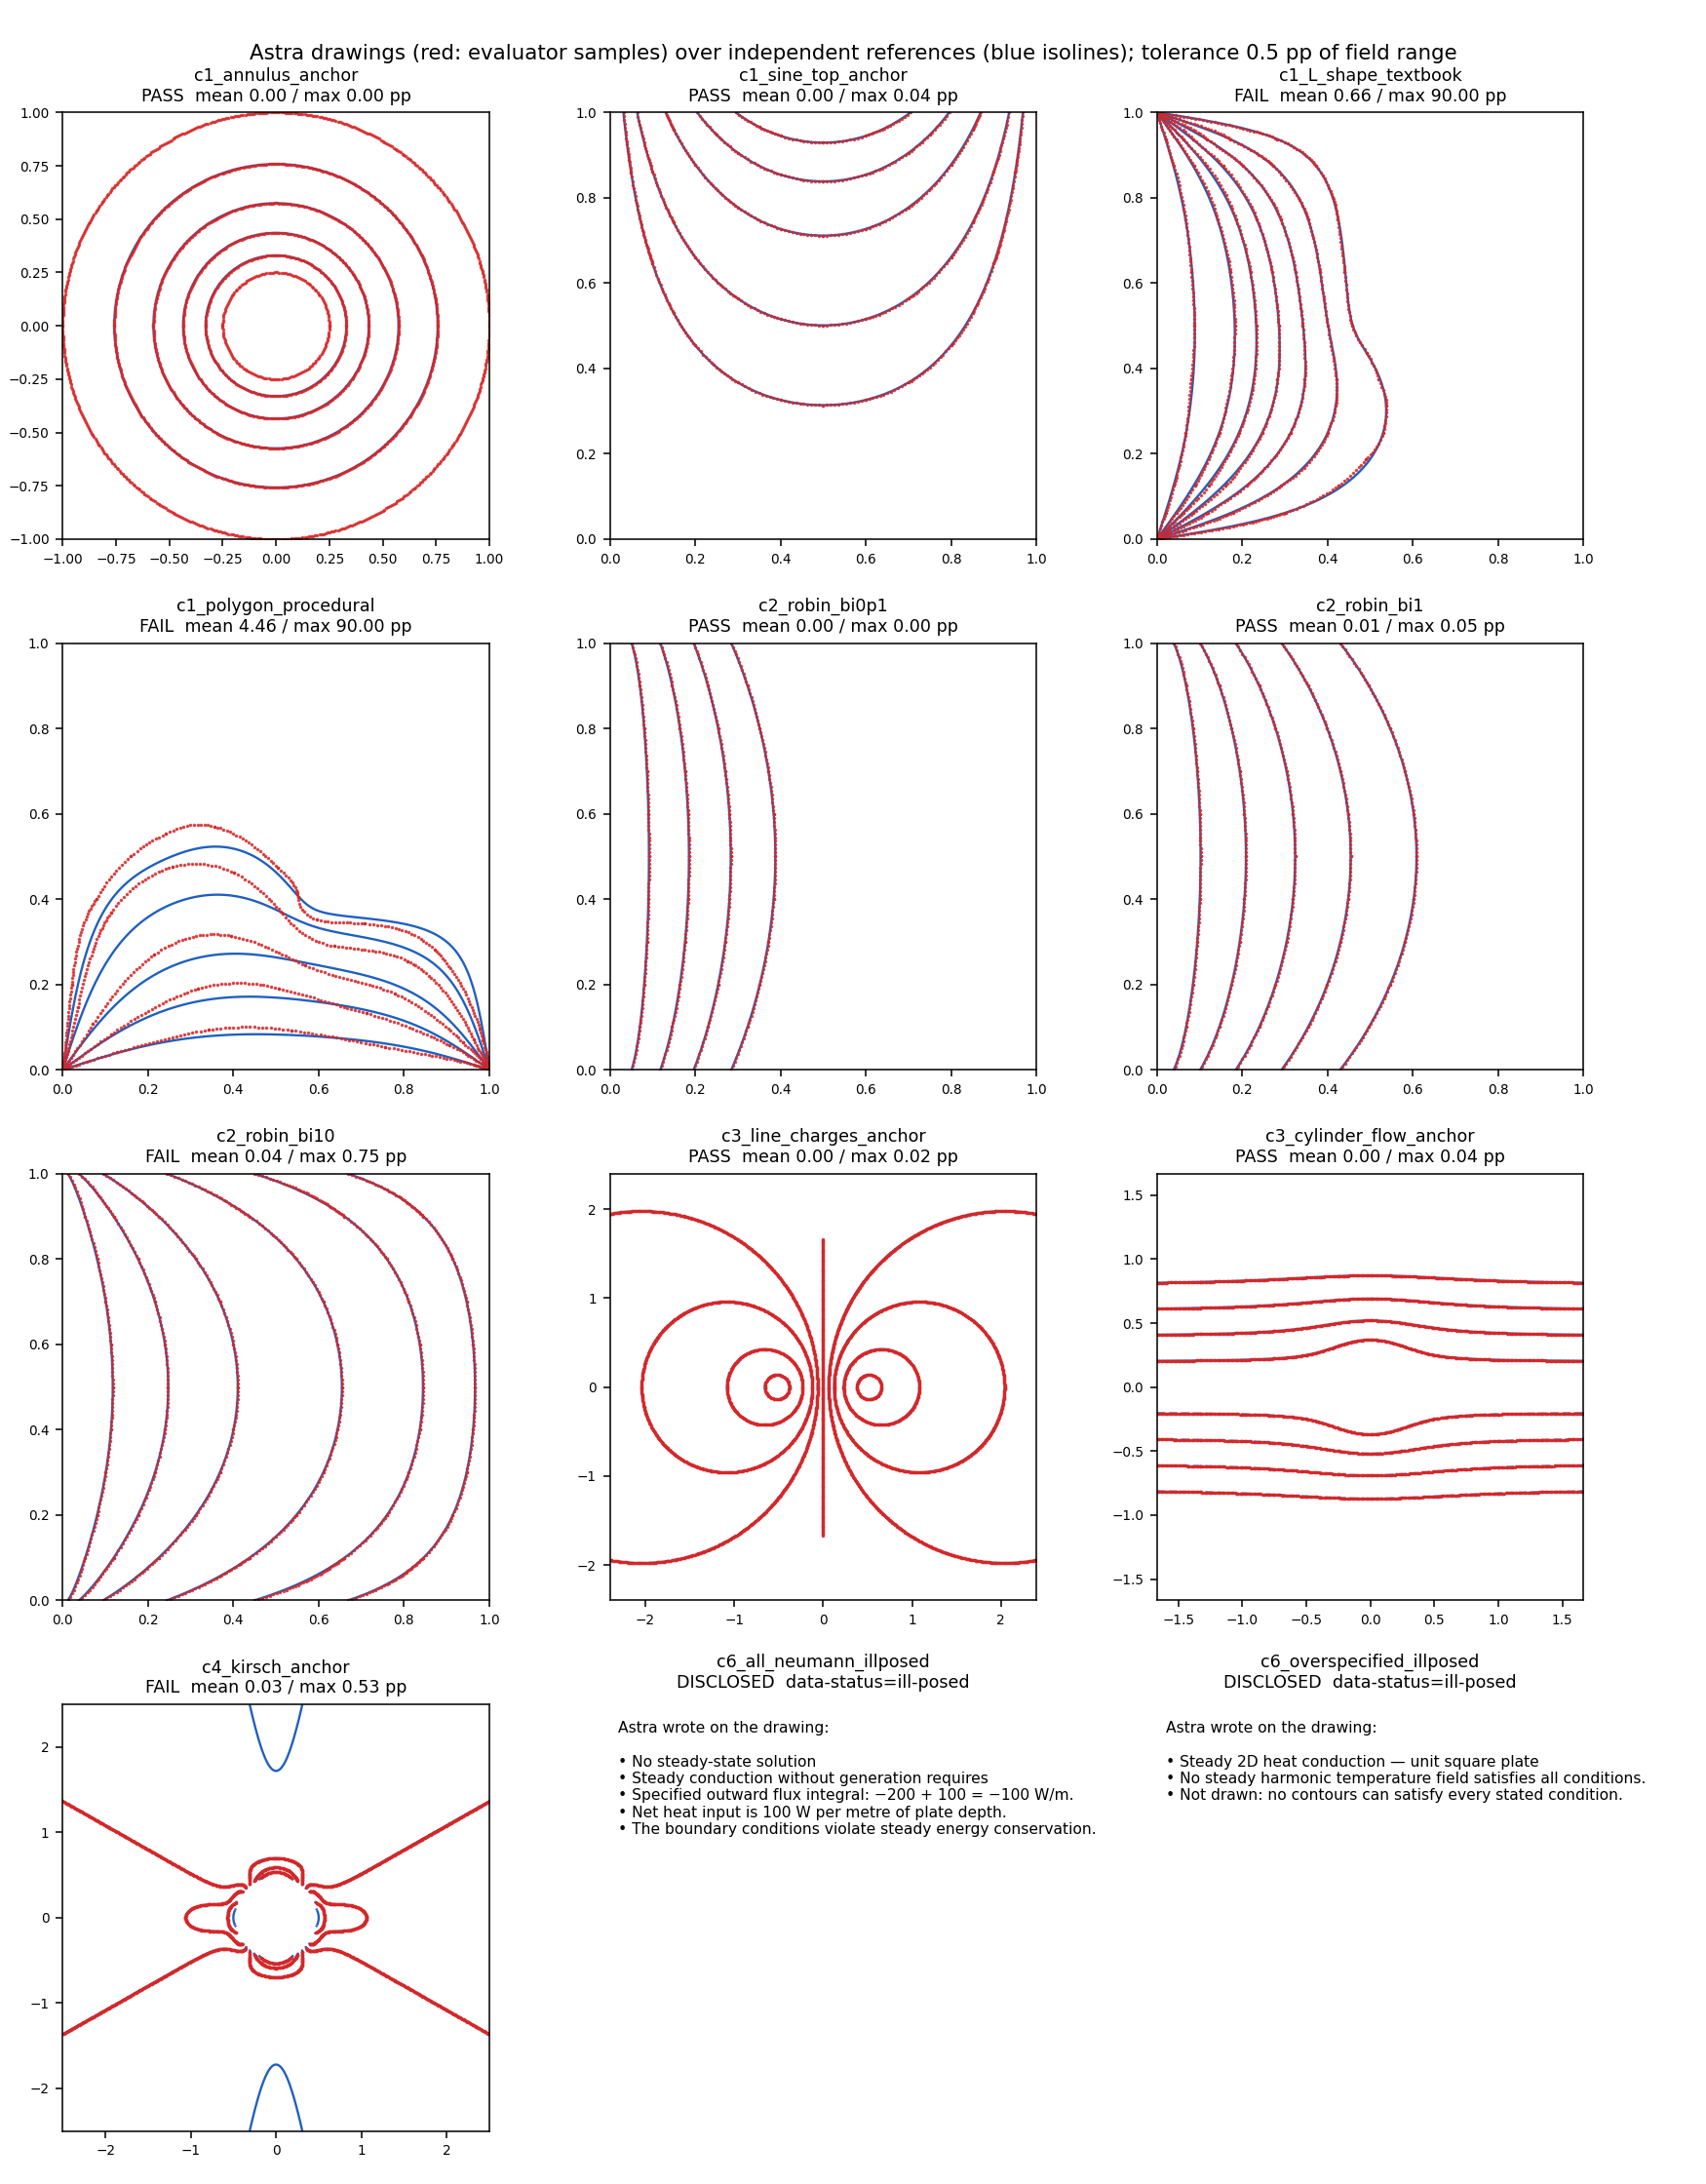
\includegraphics[width=\linewidth]{../../paper/figures/astra_hard_overlays.png}
  \caption{The model's lines (red) over the true lines (blue). Where only red is visible, the two coincide. The never-seen polygon (row 2, left) is visibly wrong; the stress plot (bottom left) is missing the blue branches at the top and bottom.}
\end{figure}

\begin{figure}[H]
  \centering
  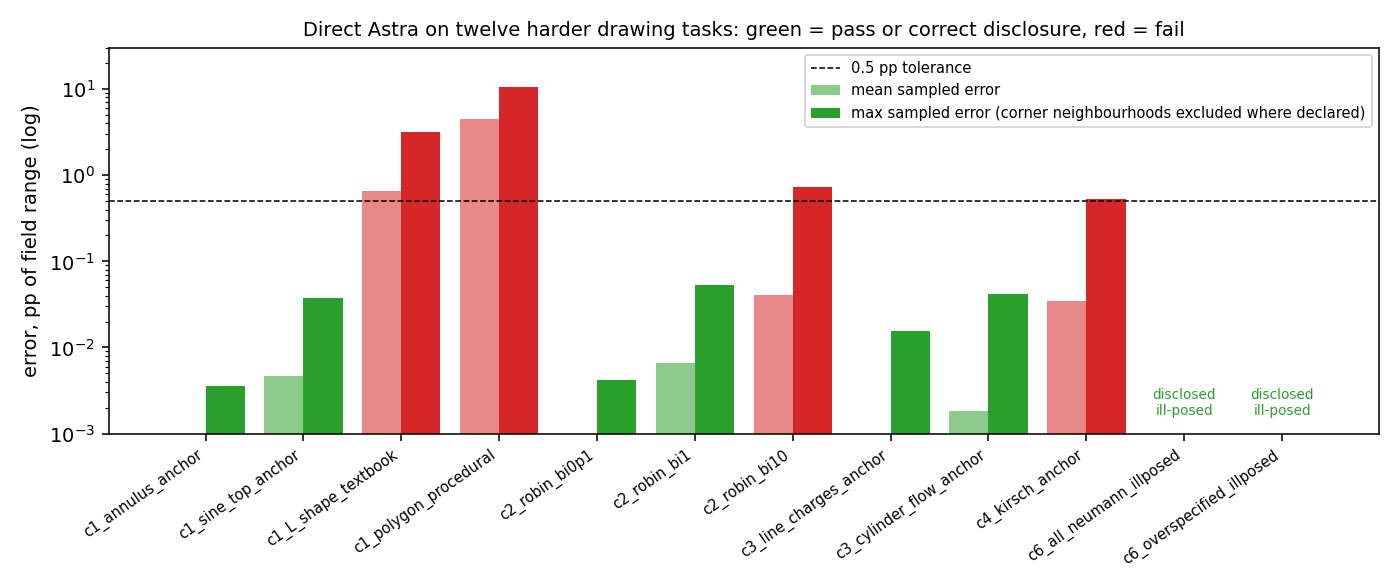
\includegraphics[width=0.9\linewidth]{../../paper/figures/astra_hard_errors.png}
  \caption{Average and worst error for each task, on a scale where each grid line is ten times the previous one. The dashed line is the pass mark.}
\end{figure}

One more finding matters: the model was asked to label each drawing as \code{solved}, \code{estimated}, \code{illustrative} or \code{ill-posed}. It called only the two exact cases ``solved''. Every drawing it called ``estimated'' really was inexact. It told the truth about its own confidence.

% =====================================================================
\section{What all this adds up to}

\begin{itemize}
  \item \textbf{The checking machinery works and is tested}, and it is hardware-independent: the same results came out of three different GPU sessions.
  \item \textbf{The first editing task was too easy.} A keyword parser, a fine-tuned small model and a frontier model all score 100\%. Nothing can be learned about ``does AI help'' from it; a harder benchmark is required before any more training.
  \item \textbf{The frontier model draws textbook physics at solver accuracy}, including problems it was previously accused of failing.
  \item \textbf{It fails on genuinely new geometry, weakens as boundary conditions get stiffer, and leaves tensor fields incomplete.} These are the places where a real solver in the loop should help.
  \item \textbf{It admits uncertainty honestly}, and it recognises impossible problems. That is exactly the behaviour the proposed ``receipts'' are meant to verify rather than trust.
  \item \textbf{Nothing here is a finished paper.} The tasks are few, sampled once, from one model on one day. The plan calls for three samples per task, several models, a budget sweep, more problem families, a checker that reads labels, and human judges of drawing quality.
\end{itemize}

\section{What happens next}

The failure classes found in C14 --- unseen geometry, strong convection, tensor stress fields, and any case where the AI must decide whether a problem is even solvable --- become the core of the benchmark. Each such case gets an FEM reference; for parametric families a PINN surrogate may replace repeated solves; and the same cases are posed in all three input modes once the image path exists. In order: build trusted references for more problem families (P01); teach the checker to read labels, units and legends (P02); assemble a benchmark of about 240 cases where keyword matching cannot succeed (P03); compare the frontier model, a solver-assisted editor, the proposed protected editor and simple template plotting on equal terms (P04); train only if that comparison shows a gap (P05); test chains of five edits where an old answer could be reused by mistake (P06); remove safety parts one at a time to see which matter (P07); and have people rate the drawings (P08). Submission deadlines for CVPR~2027 are 10, 16 and 23 November 2026.

% =====================================================================
\section*{Glossary}
\begin{description}[style=nextline]
  \item[Contour / isotherm / equipotential / streamline] A line along which one quantity (temperature, electric potential, flow) is constant.
  \item[SVG] A text-based picture format in which every line is an editable element, so a program can read and change it.
  \item[Reference solution] The trusted answer, computed by a well-checked numerical method, that a drawing is compared against.
  \item[FEM, finite differences] Two standard ways of computing physics on a computer by dividing the shape into small pieces.
  \item[pp (percentage point)] Error expressed as a fraction of the field's full range; on a 0--100\degC{} plate, 0.5 pp equals 0.5\degC.
  \item[Boundary condition] What is imposed at the edges of the shape: a fixed temperature, an insulated edge, or cooling by air (a ``Robin'' or convective condition; the Biot number measures how strong the cooling is).
  \item[Ill-posed] A problem that cannot have a solution as stated, for example more heat entering than leaving in a steady state.
  \item[PINN] A neural network trained to obey the physics equations directly, used as a fast stand-in for a solver on a family of similar problems; planned here, not yet trained.
  \item[LoRA] A cheap way of fine-tuning a large model by training a small add-on instead of all its weights.
  \item[Seed] The random starting point of a training run; repeating with several seeds checks that a result is not luck.
  \item[Astra] The frontier language model (\code{gpt-6-astra}) used through its API.
\end{description}

\section*{Where to look}
Full detail with sources: \code{output/pdf/research_overview.pdf}. Reports: \code{reports/}. Evidence: \code{runs/}. Every number in this document is copied from those files.

\end{document}
